
%(BEGIN_QUESTION)
% Copyright 2005, Tony R. Kuphaldt, released under the Creative Commons Attribution License (v 1.0)
% This means you may do almost anything with this work of mine, so long as you give me proper credit

Definer hva ``integral'' betyr når det brukes på grafen til en funksjon. Se for eksempel på denne grafen:

$$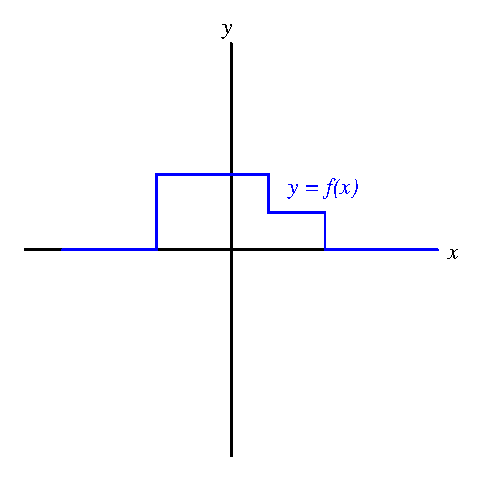
\includegraphics[width=15.5cm]{i01561x01.eps}$$

Skisser et omtrentlig plot av integralet til denne funksjonen.

\underbar{file i01561}
%(END_QUESTION)





%(BEGIN_ANSWER)

Den grafiske tolkningen av ``integral'' betyr {\it arealet} som akkumuleres under funksjonen over et gitt definisjonsområde.

$$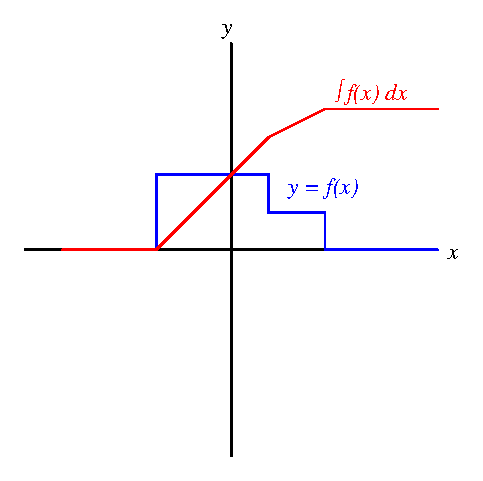
\includegraphics[width=15.5cm]{i01561x02.eps}$$

$$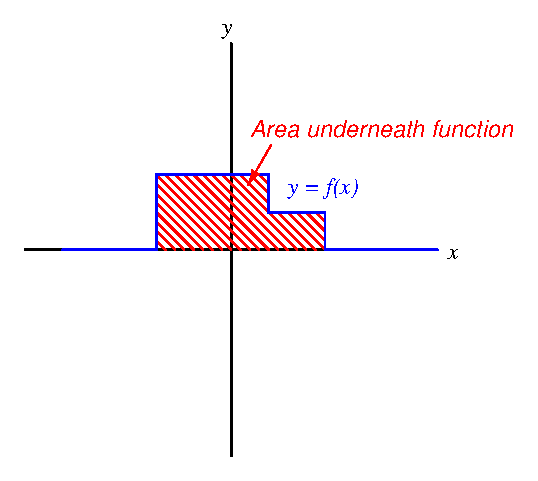
\includegraphics[width=15.5cm]{i01561x03.eps}$$

%(END_ANSWER)





%(BEGIN_NOTES)

Vanligvis synes studenter at integralbegrepet er litt vanskeligere å forstå enn begrepet derivert, selv når det tolkes grafisk. En måte å hjelpe dem over dette ``hoppet'' på er å minne om at integrasjon og derivasjon er inverse funksjoner, og deretter be dem analysere svaret ``baklengs'' (se på det røde integralplottet og hvordan den blå funksjonen er deriverten av den røde funksjonen). Tankegangen er analog med å forklare logaritmer for første gang: når vi tar logaritmen av et tall, finner vi hvilken potens vi må opphøye grunntallet i for å få dette tallet (f.eks. $\log 1000 = 3$ ; $10^3 = 1000$). Når vi finner integralet av en funksjon, finner vi hvilken annen funksjon som, når den deriveres, gir den gitte funksjonen. Dette er kjernen i det vi mener med {\it inverse funksjoner}, og det er et viktig begrep i algebra, trigonometri og kalkulus.

%INDEX% Mathematics, calculus: integral (defined in a graphical sense)

%(END_NOTES)

